%%%%%%%%%%%%%%%%%%%%%%%%%%%%%%%%%%%%%%%%%
% CN2 Labreport template
%
% License:
% CC BY-NC-SA 3.0 (http://creativecommons.org/licenses/by-nc-sa/3.0/)
%
%%%%%%%%%%%%%%%%%%%%%%%%%%%%%%%%%%%%%%%%%

\documentclass[parskip=full]{scrartcl}

\usepackage{siunitx}  % Provides the \SI{}{} command for typesetting SI units
\usepackage{graphicx} % Required for the inclusion of images
\usepackage{booktabs} % nicer tables
\usepackage[noabbrev]{cleveref} % automatic references
\usepackage{listings} % typeset code
\usepackage[backend=biber]{biblatex}
\addbibresource{referenzen.bib}

\crefname{lstlisting}{listing}{listings} % for referencing code
\Crefname{lstlisting}{Listing}{Listings} % for referencing code

\usepackage[headsepline]{scrlayer-scrpage} % header
\ohead{Group 06} % right part of header
\ihead{Assignment 3} % left part of header

\lstset{basicstyle=\ttfamily} % monospaced font in listing



%----------------------------------------------------------------------------------------
%	DOCUMENT INFORMATION
%----------------------------------------------------------------------------------------

\begin{document}
\begin{titlepage}
    \centering
    \vspace*{2cm}
    {\Huge \textbf{Communication Networks 2}}\\
    SS 2021\\
    \vspace*{1cm}
    {\Large Assignment 3}
    \\\vspace*{3cm}
    {\Large \textbf{Group 06}}\\
    \vspace*{1cm}
    {\large 
        \begin{tabular}{l c c}
            Name & Mat.Nummer \\ \hline
            Paul Kloker & 12034928 \\
            Juan Aramis Oposich & 11701238
        \end{tabular}
    }
    \\\vspace*{7cm}
    \today
\end{titlepage}

%----------------------------------------------------------------------------------------
%	SECTION 1
%----------------------------------------------------------------------------------------
\section{Task description} \label{sec:task}

%----------------------------------------------------------------------------------------
%	SECTION 2
%----------------------------------------------------------------------------------------
\section{Procedure} \label{sec:procedure}

\subsection{Host discovery with nmap} \label{subsec:nmap}
There are different techniques to discover active hosts on a network.
One of them is the use of nmap, which is a free and open source tool for network discovery and security auditing.
To find the missing host in \verb|10.0.0.0/16| the following command was used:
\begin{verbatim}
$ nmap --privileged -sn -n -T5 --min-parallelism 100 --min-hostgroup 100 
10.0.0.0/16
\end{verbatim}
To speed up the discovery process, which can take very long time in large networks, multiple options were added to the bare nmap command \verb|$ nmap 10.0.0.0/16|.
This reduced the waiting time to 23 minutes, which is still quite long. 

Table \ref{tab:nmap} shows the result of this nmap host discovery search in \verb|10.1.0.0/8| and \verb|10.0.0.0/8|.

\begin{table}[hb]
	\centering
	\begin{tabular}{|llll|}
		\hline
		\textbf{No.} & \textbf{Network} & \textbf{IP address} &\textbf{latency}  \\ 
		\hline
		1 & 10.0.0.0/8 & 10.0.4.1 &0.0075s\\
		%\hline
		2 & 10.0.0.0/8 & 10.0.4.2 &0.23s\\
		\hline
		3 & 10.0.0.0/8 & 10.0.120.1 &0.20s\\
		%\hline
		4 & 10.0.0.0/8 & 10.0.120.2 &0.0085s\\
		\hline
		5 & 10.0.0.0/8 & 10.0.132.1 &0.024s\\
		%\hline
		6 & 10.0.0.0/8 & 10.0.132.68 &0.18s\\
		\hline
		7 & 10.0.0.0/8 & 10.0.248.1 &0.78s\\
		%\hline
		8 & 10.0.0.0/8 & 10.0.248.2 &0.16s\\
		\hline
		\hline
		9 & 10.1.0.0/8 & 10.1.6.1 &0.18s\\
		%\hline
		10 & 10.1.0.0/8 & 10.1.6.110 &0.18s\\
		\hline
		11 & 10.1.0.0/8 & 10.1.7.1 &1.5s\\
		%\hline
		12 & 10.1.0.0/8 & 10.1.7.123 &0.78s\\
		\hline
	\end{tabular}
	\caption{Discovered IP addresses}
	\label{tab:nmap}
\end{table}

Later research and additional information showed that the 6th found IP address \verb|10.0.132.68| belongs to the missing host. 


\subsection{Ping measurements} \label{subsec:ping}
To identify which IP address belongs to the landline and satellite host a simple ping command was sent out to the according DNS names.
\verb|landline.cn2lab.cn.tuwien.ac.at| was resolved to \verb|10.1.6.110| and \verb|satellite.cn2lab.cn.tuwien.ac.at| to \verb|10.1.7.123|.

In order to obtain information about the network topology and the Round Trip Time (RTT) and loss rate of each host, the ping command was used as well.
For each IP address from \cref{tab:nmap} the following command was adapted and executed:
\begin{verbatim}
$ ping -c 50 -R 10.1.7.123 > 10_1_7_123.txt
\end{verbatim}
This delivered 50 individual measurements of the RRT which were then saved to a text file and are discussed in \cref{sec:data}.

With the \verb|-R| the record route option was activated.
That means all internet modules that route this message add their IP address to the IP option field.
This method is better than just using the command \verb|traceroute| because here the reverse path is recorded as well.

Some recorded routes show that the reverse path can be different from the forward path. 
This is for example the recorded route of the satellite host:
\begin{verbatim}
RR:  pc18.cn2lab.cn.tuwien.ac.at (192.168.88.118)
     10.0.120.2 (10.0.120.2)
     10.0.248.2 (10.0.248.2)
     10.1.7.1 (10.1.7.1)
     satellite.cn2lab.cn.tuwien.ac.at (10.1.7.123)
     satellite.cn2lab.cn.tuwien.ac.at (10.1.7.123)
     10.0.4.2 (10.0.4.2)
     border.cn2lab.cn.tuwien.ac.at (192.168.88.2)
     pc18.cn2lab.cn.tuwien.ac.at (192.168.88.118)
\end{verbatim}

\subsection{Network topology}
Using the data of the nmap and ping commands, the network topology could be identified and a network diagram created which can be seen in \cref{fig:topology}.
\begin{figure}[!ht]
	\centering % centering figure 
	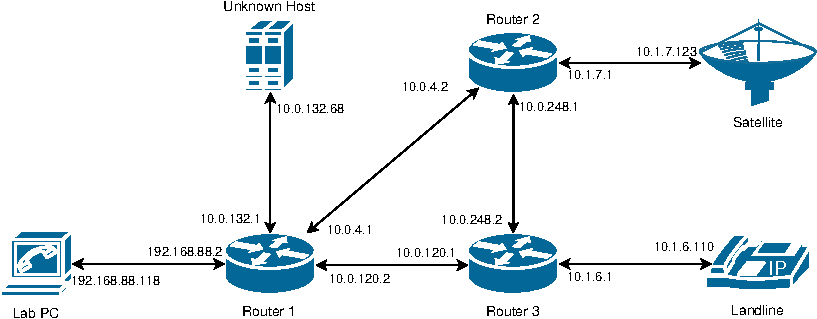
\includegraphics[width=\textwidth]{images/topology.pdf} % importing figure
	\caption{Network diagram} 
	\label{fig:topology} % labeling to refer it inside the text
\end{figure}
Table \ref{tab:routing} shows the routing tables of the three routers. 
Some entries could not be identified by just using the ping command on the lab pc.

\begin{table}[hb]
	\centering

	\begin{tabular}{lll}
		\toprule
		\textbf{router} & \textbf{destination} & \textbf{via}  \\ \midrule
		r1 & 10.0.4.0/24 & 10.0.4.1 \\
		r1 & 10.0.120.0/24 & 10.0.120.2 \\
		r1 & 10.0.132.0/24 & 10.0.132.1 \\
		r1 & 10.0.248.0/24 & 10.0.120.2 \\
		r1 & 10.1.6.0/24 & 10.0.120.2 \\
		r1 & 10.1.7.0/24 & 10.0.120.2 \\
		r1 & 192.168.88.0/24 & 192.168.88.2\\
		\midrule
		r2 & 10.0.4.0/24 & - \\
		r2 & 10.0.120.0/24 & 10.0.120.1 \\
		r2 & 10.0.132.0/24 & - \\
		r2 & 10.0.248.0/24 & 10.0.248.2 \\
		r2 & 10.1.6.0/24 & 10.1.6.1 \\
		r2 & 10.1.7.0/24 & - \\
		r2 & 192.168.88.0/24 & 10.0.120.1\\
		\midrule
		r3 & 10.0.4.0/24 & 10.0.4.2 \\
		r3 & 10.0.120.0/24 & - \\
		r3 & 10.0.132.0/24 & - \\
		r3 & 10.0.248.0/24 & 10.0.248.1 \\
		r3 & 10.1.6.0/24 & - \\
		r3 & 10.1.7.0/24 & 10.0.7.1 \\
		r3 & 192.168.88.0/24 & 10.0.4.2\\
		\bottomrule
	\end{tabular}
	\caption{Routing table for network A}
	\label{tab:routing}
\end{table}
\clearpage
\section{Data analysis and comparison} \label{sec:data}
- Welche daten liefert ping

- Grafische Darstellung (besonders Vergleich von Landline und Satellite)

- Vergleich mit den gemessenen Daten von Task 2

One of the most important as metrics of a real-time communication like VoIP is the end-to-end ($T_{EE}$) delay. In this context the ITU-T recommendation G.114 has classified the user acceptance for end-to-end delays in a VoIP call \cite{ITU-TRecommendationG.114}:

\begin{table}[hb]
	\centering
	\begin{tabular}{ll}
		\toprule
		\textbf{End-to-End delay} & \textbf{User experience} \\ \midrule
			$T_{EE} < 150$ & acceptable for all users \\
			$150 < T_{EE} < 300$ & noticeable quality degradation, but still acceptable for most users\\
			$T_{EE} \geq 300$ & not acceptable\\
			\bottomrule
		\end{tabular}
		\caption{Delay to user experience}
		\label{tab:delayEnd2End}
	\end{table}
	
To determine the one-way transmission time it is mandatory to divide the RRT value by two.

\begin{figure}[!ht]
	\centering % centering figure 
	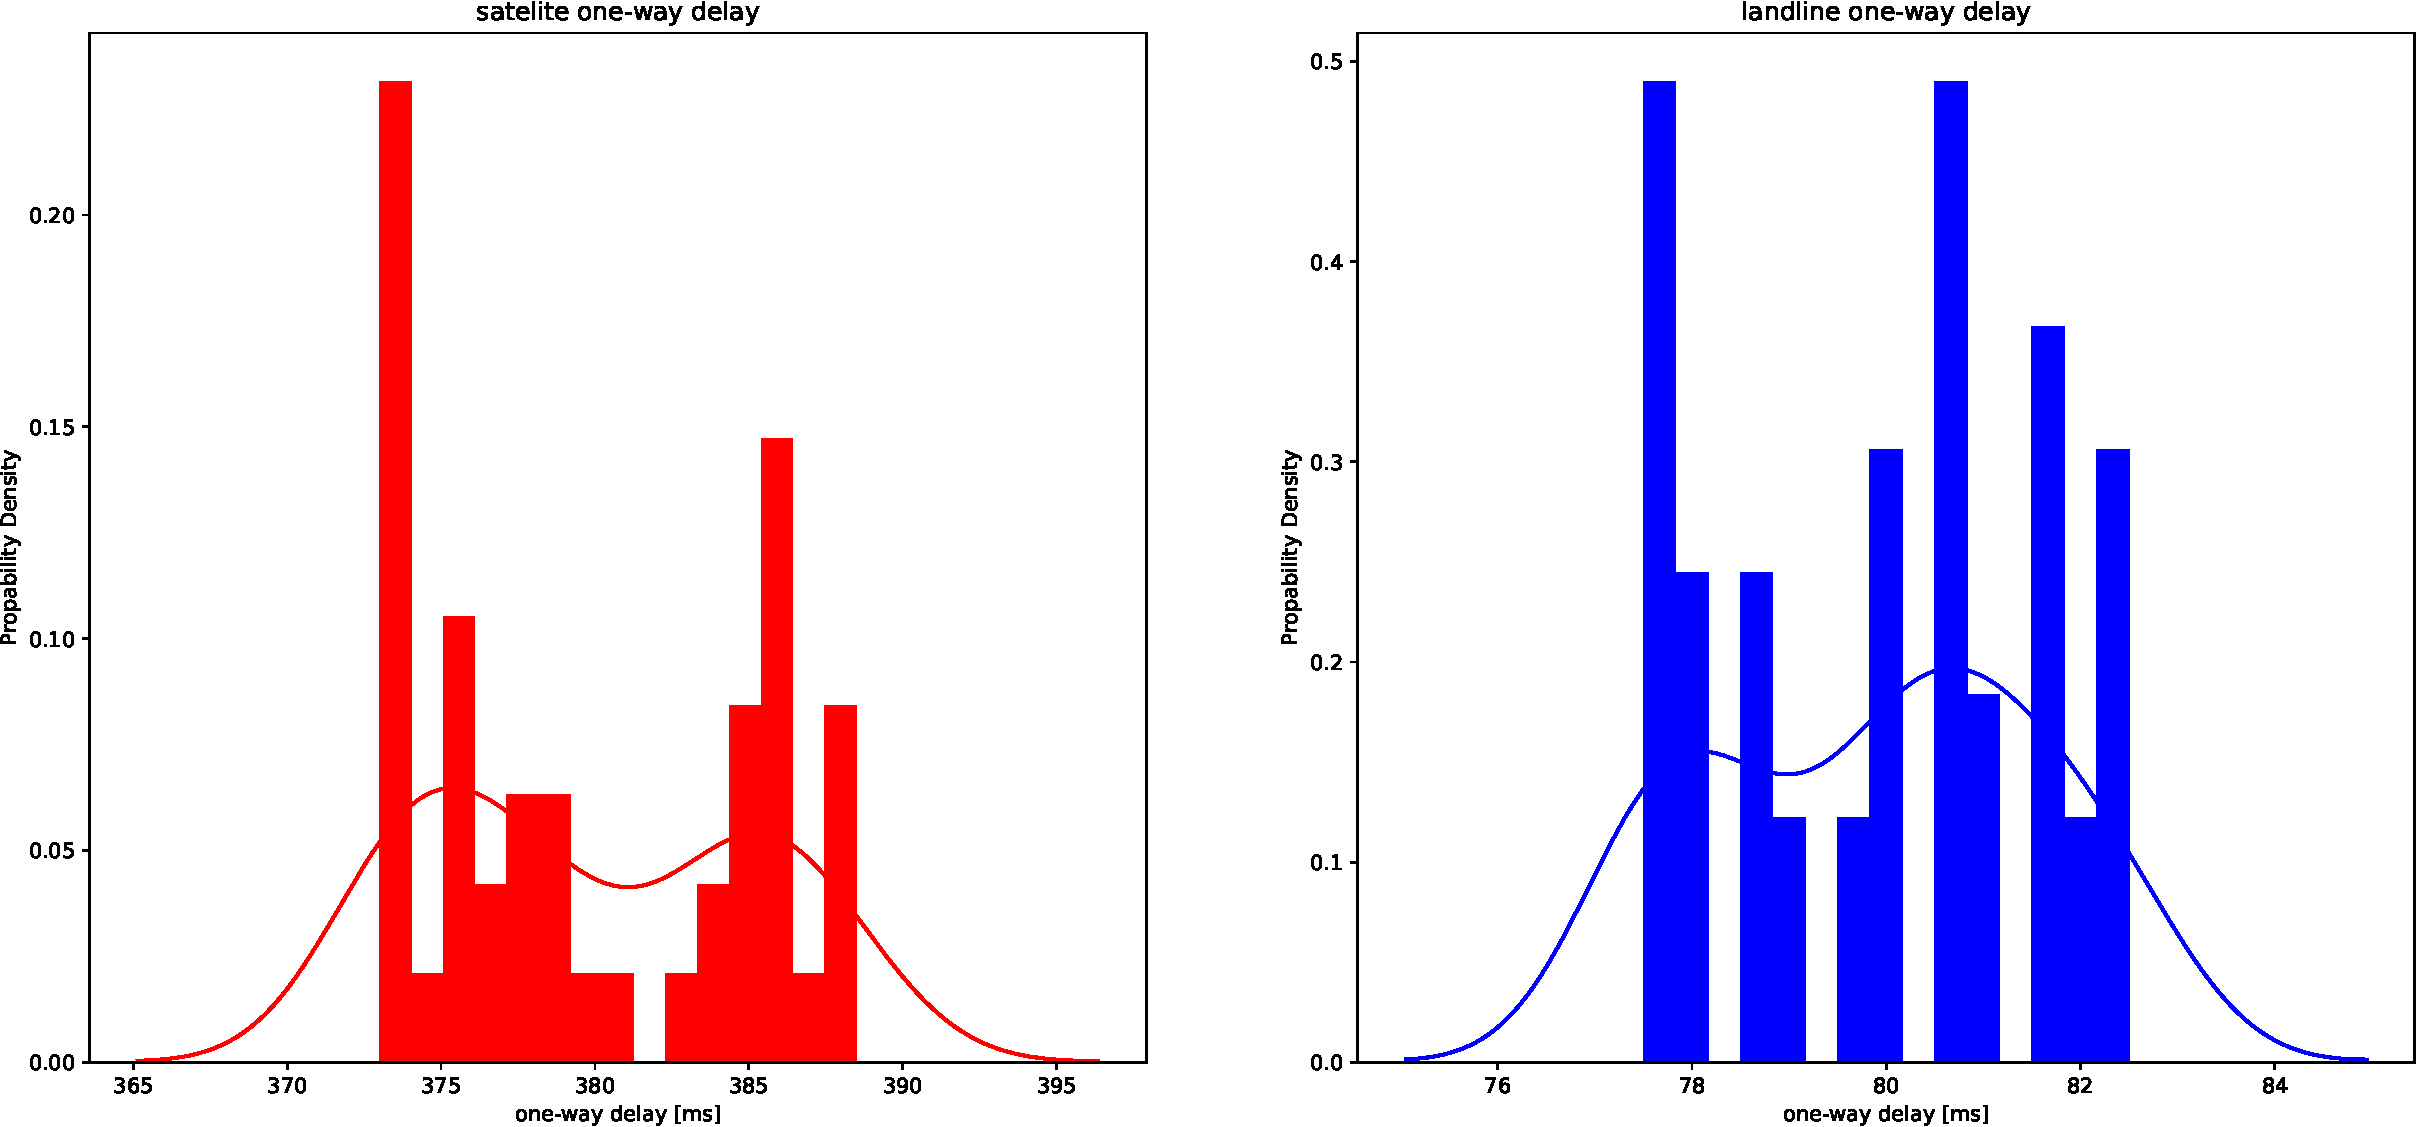
\includegraphics[width=\textwidth]{images/oneWayDelay.pdf} % importing figure
	\caption{Propobility density of one way delay} 
	\label{fig:one-way-delay} % labeling to refer it inside the text
\end{figure}



%----------------------------------------------------------------------------------------
%	SECTION 3
%----------------------------------------------------------------------------------------
\newpage
\section{Conclusion}

%----------------------------------------------------------------------------------------
%	SECTION X
%---------------------------------------------------------------------------------------

\printbibliography

\end{document}
